\subsubsection{Faster R-CNN}
Trước khi đi vào Faster R-CNN, ở báo cáo này nhóm sẽ giới thiệu sơ lược về các mô hình cùng thuộc gia đình R-CNN trong bài toán object detection bao gồm: R-CNN, Fast R-CNN.

\paragraph{R-CNN (Region with CNN feature)\\}

R-CNN \cite{rcnn} là một thuật toán two-stage để phát hiện vật thể. Ý tưởng của bài toán R-CNN khá đơn giản:
\begin{itemize}[noitemsep, topsep=0pt, leftmargin=1.25em, label={$-$}]
    \item Bước 1: Dùng thuật toán Selective Search để lấy ra khoảng 2000 bounding box trong input mà có khả năng chứa đối tượng.
    \item Bước 2: Với mỗi vùng bounding box ta xác định nó là đối tượng nào.
\end{itemize}

Nói về thuật toán Selective Search thì đây là thuật toán đề xuất khu vực cho các công việc Object Detection. Nó chia ảnh thành các phần với với mật độ điểm ảnh dựa trên phương pháp phân đoạn dựa trên đồ thị của Felzenszwalb và Huttenlocher.Sau đó, Selective Search sử dụng các phần đã chia được và thực hiện các bước sau:
\begin{enumerate}[topsep=0pt,itemsep=-1ex,partopsep=1ex,parsep=1ex]
    \item Thêm các bounding box tương ứng với phần đã được phân đoạn vào danh sách các region proposals (vùng đề xuất)
    \item Nhóm các phân đoạn liền kề dựa trên sự tương đồng
    \item Quay lại bước 1
\end{enumerate}

Tại mỗi lần lặp lại, các phân đoạn lớn hơn được hình thành và thêm vào danh sách các region proposals.

\begin{figure}[h!]
  \centering
  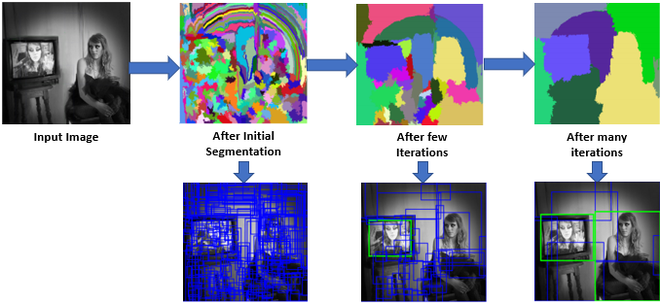
\includegraphics[scale=0.58]{graphics/selective search.png}
  \caption{Sử dụng Selective Search để tạo ra các bounding box}
\end{figure}

Kiến trúc của R-CNN gồm 3 thành phần:
\begin{itemize}[noitemsep, topsep=0pt, leftmargin=1.25em, label={$-$}]
    \item Vùng đề xuất hình ảnh: có tác dụng tạo và trích xuất các vùng đề xuất chứa vật thể được bao bởi các bounding box. 
    \item Trích xuất đặc trưng (feature extractor): trích xuất các đặc trưng giúp nhận diện hình ảnh từ các region proposals thông qua các mạng convolutional neural network (CNN).
    \item Phân loại (classifier): dựa vào input là các features ở phần trước để phân loại hình ảnh chứa trong region proposal về đúng nhãn.
\end{itemize}
\graphicspath{{figures/}}
\begin{figure}[h!]
  \centering
  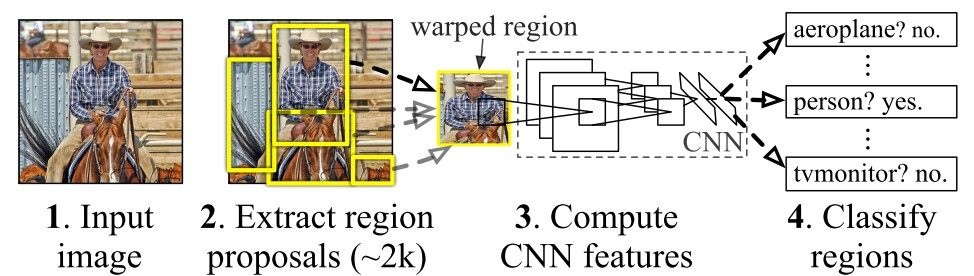
\includegraphics[scale=0.45]{graphics/RCNN.jpg}
  \caption{Sơ đồ pipeline xử lý trong mô hình R-CNN}
\end{figure}

Một trong những cải tiến của R-CNN là sử dụng mô hình SVM (Support Vector Machine) để phân loại các vùng đề xuất và mô hình hồi quy (bounding box regression) riêng biệt để dự đoán vị trí. Qua đó, mô hình R-CNN có khả năng đạt được kết quả chính xác trong việc nhận diện và định vị vật thể trong ảnh.\\
Tuy R-CNN đạt được kết quả khá tốt trong bài toán Object Detection, tuy nhiên, quá trình huấn luyện và dự đoán của mô hình này khá chậm do cần phải xử lý mỗi region proposal một cách độc lập như ở hình trên cần phải xử lý khoảng 2000 vùng đề xuất cho mỗi hình ảnh tại thời điểm thử nghiệm.

\paragraph{Fast R-CNN\\}
Dựa trên thành công của R-CNN, Ross Girshick (lúc này đã chuyển sang Microsoft Research) và các cộng sự của ông đã đề xuất một phương pháp mở rộng để giải quyết các hạn chế của R-CNN trong một bài báo vào năm 2015 với tiêu đề ngắn gọn là Fast R-CNN \cite{fastrcnn}.

Trong bài báo, nhóm tác giả đã chỉ ra những hạn chế của R-CNN đó là:
\begin{itemize}[noitemsep, topsep=0pt, leftmargin=1.25em, label={$-$}]
    \item Quá trình huấn luyện qua một pipeline phức tạp: R-CNN yêu cầu một pipeline gồm nhiều bước, bao gồm chuẩn bị dữ liệu, huấn luyện mạng CNN và các mô hình phụ trợ như SVM. Quá trình này phức tạp và tốn nhiều thời gian và công sức.
    \item Chi phí training tốn kém về số lượng bounding box và thời gian huấn luyện: R-CNN đòi hỏi huấn luyện mạng CNN trên một lượng lớn region proposal cho mỗi hình ảnh. Điều này dẫn đến việc tốn kém về tài nguyên tính toán và thời gian huấn luyện.
    \item Phát hiện đối tượng chậm: Do quá trình phải xử lý một lượng lớn region proposal, R-CNN không đảm bảo tốc độ phát hiện vật thể trong thời gian thực (real-time).
\end{itemize}
\graphicspath{{figures/}}
\begin{figure}[h!]
  \centering
  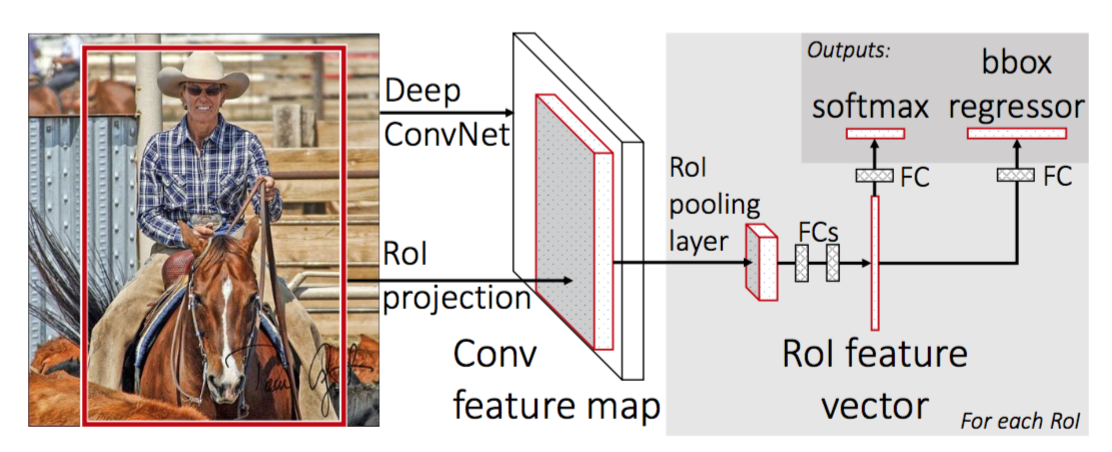
\includegraphics[scale=0.35]{graphics/fast-RCNN.png}
  \caption{Sơ đồ pipeline xử lý trong mô hình Fast R-CNN}
\end{figure}
Cách tiếp cận của mô hình Fast R-CNN khá giống với R-CNN tuy nhiên, thay vì đưa các vùng đề xuất (region proposals) qua mạng CNN, Fast R-CNN đưa hình ảnh đầu vào qua một mạng CNN duy nhất để trích xuất ra được convolutional feature map. Điều này giúp tái sử dụng đặc trưng cho toàn bộ ảnh và giảm thiểu thời gian tính toán so với R-CNN. Từ convolution feature map, Fast R-CNN sử dụng kỹ thuật RoI Pooling để chuyển đổi các vùng đề xuất có kích thước và hình dạng khác nhau thành các vùng có kích thước cố định. Sau đó, các vùng này được đưa qua các lớp Fully-Connected để phân loại và dự đoán vị trí. Cuối cùng mô hình chia thành hai đầu ra, một đầu ra cho dự đoán nhãn thông qua một softmax layer và một đầu ra khác dự đoán bounding box (kí hiệu là bbox) dựa trên hồi qui tuyến tính. Quá trình này sau đó được lặp lại nhiều lần cho mỗi vùng RoI trong một hình ảnh.

Ở trên, ta có đề cập tới một thuật ngữ là RoI Pooling. Region of Interest (RoI) pooling là một dạng của pooling layer. Điểm khác so với max pooling hay average pooling là bất kể kích thước của tensor input, RoI pooling luôn cho ra output có kích thước cố định được định nghĩa trước. Nó được sử dụng để biến đổi vùng đề xuất có kích thước khác nhau thành các vùng đặc trưng có kích thước cố định, giúp thuận tiện cho việc sử dụng các mạng nơ-ron fully connected.

Giả sử input của RoI pooling có kích thước m*n, trong đó m là chiều cao và n là chiều rộng của vùng đề xuất. Output của ROI pooling có kích thước h*k, với h và k thường được chọn nhỏ, ví dụ như 7*7.

Cách thức hoạt động của RoI pooling như sau:
\begin{enumerate}[topsep=0pt,itemsep=-1ex,partopsep=1ex,parsep=1ex]
    \item Chia vùng đề xuất thành h x k ô con có kích thước gần bằng nhau. Số ô con hình thành từ việc chia này sẽ bằng h*k.
    \item Đối với mỗi ô con, tìm giá trị tối đa (max pooling) từ vùng tương ứng trên input.
    \item Gom các giá trị tối đa này thành một vectơ đặc trưng có kích thước h*k.
\end{enumerate}

Qua quá trình này, RoI pooling thu được các vùng đặc trưng có kích thước cố định h*k, không phụ thuộc vào kích thước ban đầu của vùng đề xuất.

Sự khác biệt giữa Fast R-CNN và R-CNN là ở cách thức thực hiện feature map và tính toán trên region proposals. Trong Fast R-CNN, feature map được tạo từ cả ảnh đầu vào, và sau đó các region proposals được trích xuất từ feature map. Trái lại, R-CNN tách riêng các region proposal và thực hiện CNN trên từng region proposal.

\graphicspath{{figures/}}
\begin{figure}[h!]
  \centering
  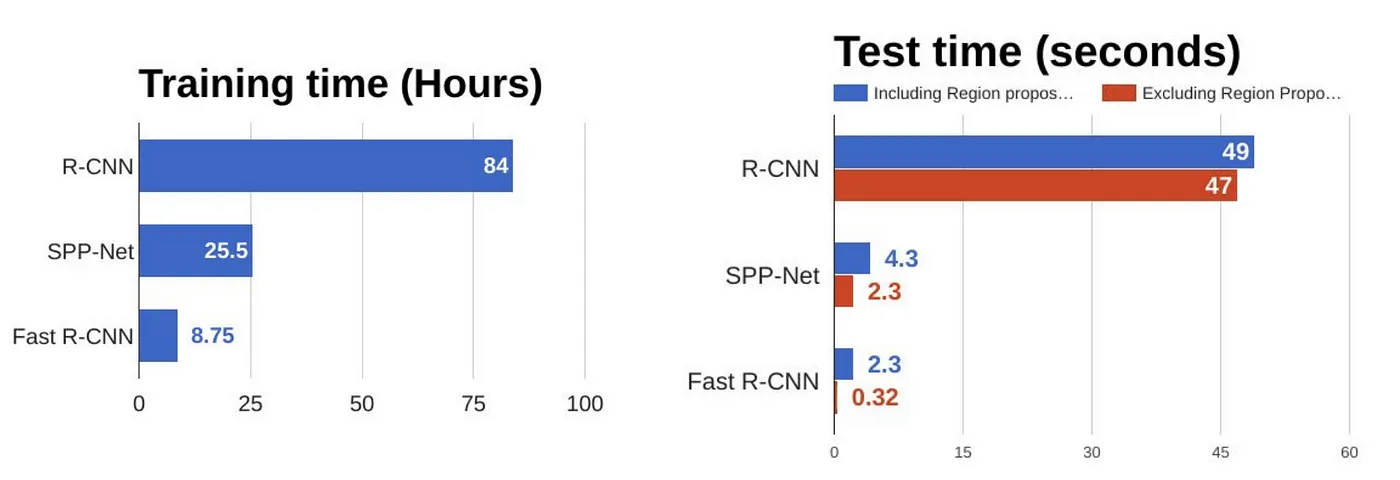
\includegraphics[scale=0.3]{graphics/Fast R-CNN compare.png}
  \caption{Biểu đồ so sánh thời gian giữa R-CNN, SPP-Net và Fast R-CNN \cite{compare}}
\end{figure}

Dựa vào hình trên, ta có thể thấy rằng Fast R-CNN mang lại kết quả tốt, với hiệu suất vượt trội so với R-CNN trong quá trình huấn luyện và thực nghiệm. Khi xem xét hiệu suất của Fast R-CNN trong thời gian thực nghiệm, việc bao gồm các vùng đề xuất làm chậm thuật toán một cách đáng kể so với việc không sử dụng các vùng đề xuất. Do đó, vùng đề xuất trở thành bottleneck trong mô hình Fast R-CNN, ảnh hưởng đến hiệu suất của nó.

\paragraph{Faster R-CNN\\}
Kiến trúc mô hình đã được cải thiện hơn nữa về cả tốc độ huấn luyện và phát hiện được đề xuất bởi Shaoqing Ren và các cộng sự tại Microsoft Research trong bài báo năm 2016 có tiêu đề Faster R-CNN: Towards Real-Time Object Detection with Region Proposal Networks \cite{fastercnn}. Dịch nghĩa là “Faster R-CNN: Hướng tới phát hiện đối tượng theo thời gian thực với các mạng đề xuất khu vực”.

Mặc dù Faster R-CNN là một mô hình đơn lẻ duy nhất nhưng nó kết hợp 2 modules:
\begin{itemize}[noitemsep, topsep=0pt, leftmargin=1.25em, label={$-$}]
    \item Mạng đề xuất khu vực (Region Proposal Network): Mạng CNN để đề xuất các vùng và loại đối tượng cần xem xét trong vùng
    \item Fast R-CNN: Mạng CNN để trích xuất các features từ các region proposal và trả ra các bounding box và nhãn
\end{itemize}

\subparagraph{Region Proposal Network (RPN)\\}
Faster R-CNN không dùng thuật toán Selective Search để lấy ra các region proposal, mà nó thêm một mạng CNN mới mà trong bài báo trên tác giả gọi là Region Proposal Network (RPN) để tìm các region proposal.

\graphicspath{{figures/}}
\begin{figure}[h!]
  \centering
  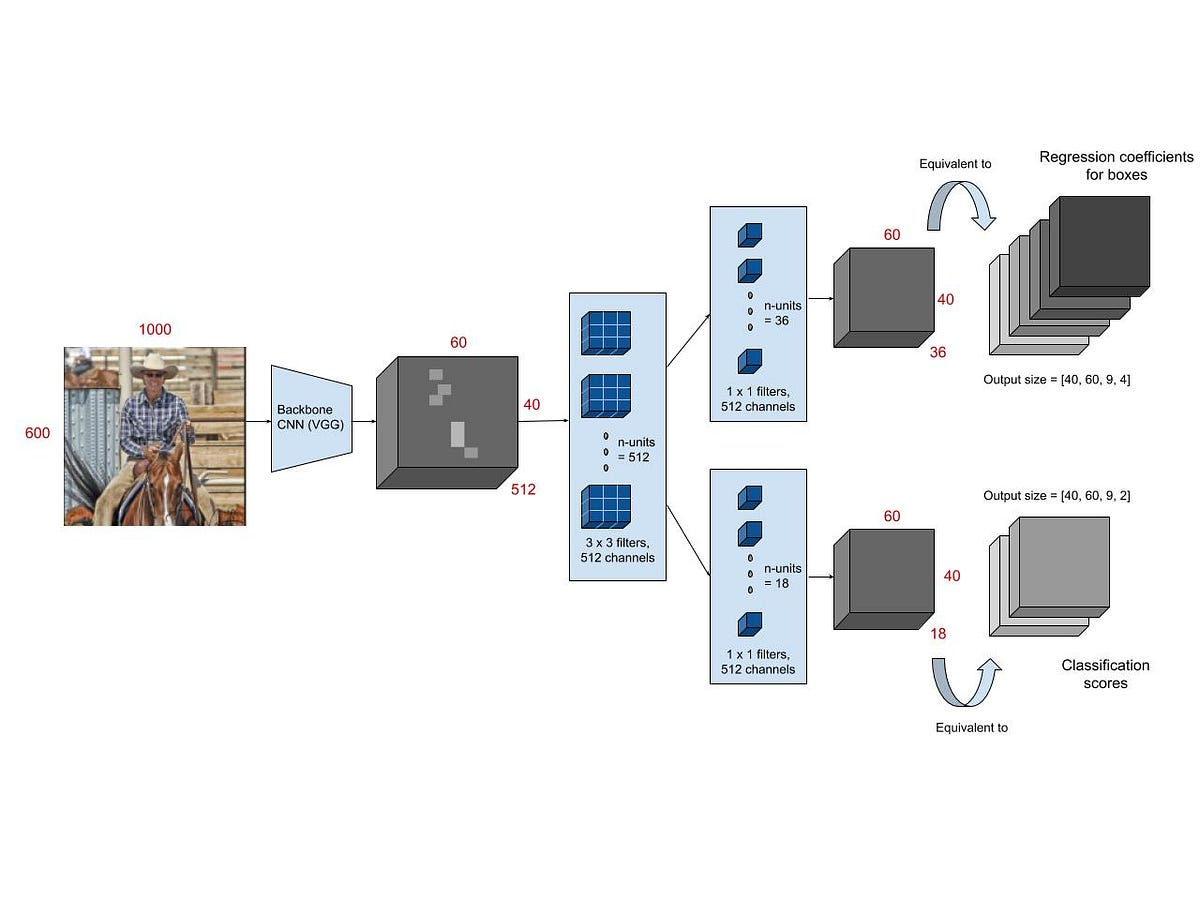
\includegraphics[scale=0.3]{graphics/rpn.jpg}
  \caption{Cấu trúc của Region Proposal Networks (RPN)}
\end{figure}

Về cơ bản thì ta có thể thấy rằng mô hình Faster RCNN kế thừa từ Fast RCNN bằng việc thay Selective Search bằng lớp RPN. 
RPN bắt đầu bằng việc đưa hình ảnh đầu vào vào backbone convolutional neural network. Ảnh đầu vào được thay đổi kích thước sao cho chiều rộng ngắn nhất là 600px và chiều dài không vượt quá 1000px.

Đầu ra của backbone network là một feature map thường nhỏ hơn nhiều so với ảnh đầu vào tùy thuộc vào bước đi (stride) của backbone network, nhưng vẫn giữ lại thông tin về các đặc trưng quan trọng của ảnh. Đối với hai backbone network được sử dụng trong bài báo (VGG, ZF-Net), bước đi của mạng là 16. Điều này có nghĩa là hai điểm liên tiếp trong đặc trưng đầu ra của backbone network tương ứng với hai điểm cách nhau 16 pixels trên ảnh đầu vào.

Trên feature map, RPN sử dụng một cửa sổ trượt (sliding window) có kích thước cố định để duyệt qua từng vị trí trên feature map. Tại mỗi vị trí, RPN áp dụng một số anchors, có thể hiểu là các pre-defined boxes được định nghĩa trước lúc khi huấn luyện mô hình, để dự đoán xem vùng đó có chứa vật thể hay không và điều chỉnh kích thước của anchors để chính xác phù hợp với vật thể. Hình dưới đây cho thấy 9 anchor có tỷ lệ khía cạnh và kích thước khác nhau được đặt trên ảnh đầu vào cho một điểm pixel A trên bản đồ đặc trưng (feature map) đầu ra. Đối với bộ dữ liệu PASCAL, các anchor được sử dụng có 3 tỷ lệ kích thước là \(128^2\), \(2256^2\), \(512^2\) và 3 tỷ lệ khía cạnh là 1:1, 1:2 và 2:1.
\graphicspath{{figures/}}
\begin{figure}[h!]
  \centering
  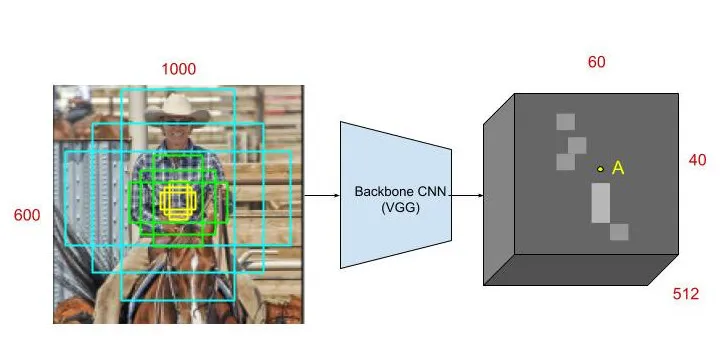
\includegraphics[scale=0.45]{graphics/anchor.png}
  \caption{Các anchors có thể có trong hình ảnh đầu vào ở một vị trí tương ứng với điểm A trong feature map}
\end{figure}

Các anchor thông thường được định nghĩa với 3 anchor size và 3 anchor ratio khác nhau và do đó có tổng cộng k = 9 anchor (k cũng có thể khác 9). Ví dụ feature map đầu ra đang là 37x50x256 thì tổng số anchor box sẽ là 37x50x9=16650. Các anchor box được đưa vào thuật toán NMS để chắc chắn rằng các vùng dự đoán không chồng chéo lên nhau. Kết thúc RPN sẽ được đưa vào lớp RoI Pooling (đã đề cập ở Fast R-CNN) để cố định kích thước đầu vào các feature map trước khi đưa vào mạng gồm nhánh fully connected.

Các anchor này được gán cho các nhãn là positive hoặc negative (object hoặc background) dựa vào diện tích trùng lặp hay IoU (đã đề cập ở phần độ đo) với ground-truth bounding box theo quy tắc sau:
\begin{itemize}[noitemsep, topsep=0pt, leftmargin=1.25em, label={$-$}]
    \item Các anchor có tỉ lệ IoU lớn nhất với ground-truth box sẽ được coi là positive
    \item Các anchor có tỉ lệ IoU \(\geq 0.7\) sẽ được coi là positive
    \item Các anchor có tỉ lệ IoU < 0.3 sẽ được coi là negative (background)
    \item Các anchor nằm trong khoảng \(0.3 \leq x < 0.7\) sẽ được coi là neutral (trung tính) là sẽ không được sử dụng trong quá trình huấn luyện mô hình
\end{itemize}
\graphicspath{{figures/}}
\begin{figure}[h!]
  \centering
  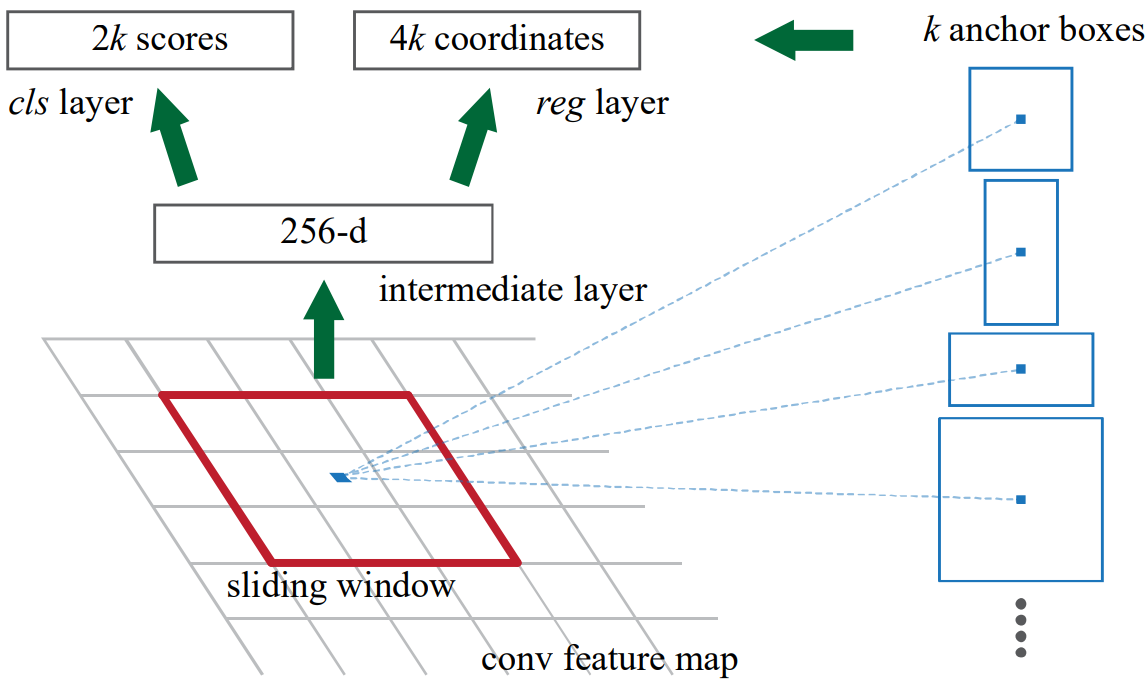
\includegraphics[scale=0.45]{graphics/rpn.png}
  \caption{Region Proposal Network (RPN)}
\end{figure}

Với mỗi vùng đề xuất kích thước nxn, một vector đặc trưng (có độ dài 256 với ZF net và 512 với VGG-16 net) được trích xuất. Vector này được đưa qua 2 lớp mạng fully connected:
\begin{enumerate}[topsep=0pt,itemsep=-1ex,partopsep=1ex,parsep=1ex]
    \item Lớp fully connected (FC) đầu tiên được gọi là "cls" đóng vai trò là một bộ phân loại nhị phân. Nó dùng để tính độ tin cậy (objectness score) cho mỗi region proposal, tức là xác định xem vùng đó có chứa đối tượng hay chỉ là phần nền (background).
    \item Lớp FC thứ hai được gọi là "reg" và trả về một vector 4 chiều, xác định các tọa độ bounding box của region proposal. Vector này cung cấp thông tin về vị trí và kích thước của đối tượng trong vùng đề xuất.
\end{enumerate}
Với binary object classification sẽ cho đầu ra là 2k channel output với k ở đây là tổng số lượng anchor box với 2 ở đây là vì chúng ta chỉ quan tâm box đó có chưa đối tượng hay không. Với bounding box regression thì có 4k channel output, với 4 là đặc trưng cho 4 tọa độ offset (x, y, w, h). 

\subparagraph{Hàm loss\\}
Trong paper thì tác giả có sử dụng hàm smooth-L1 loss, hàm loss của RPN là loss tổng của classification và regression.
\begin{equation*}
    L({p_i}, {t_i}) = \frac{1}{N_{cls}}\sum_i L_{cls}(p_i, p^*_i) + \lambda \frac{1}{N_{reg}}\sum_i p^*_i L_{reg}(t_i, t^*_i)
\end{equation*}
Trong đó:
\begin{itemize}[noitemsep, topsep=0pt, leftmargin=1.25em, label={$-$}]
    \item i là chỉ số của một anchor trong một mini-batch và \(p_i\) là xác suất dự đoán của anchor i là một đối tượng.
    \item \(p^*_i\) có giá trị 1 nếu anchor là positive (chứa đối tượng), và có giá trị 0 nếu anchor là negative (không chứa đối tượng).
    \item \(t_i\) là một vector biểu diễn 4 thông số của bounding box dự đoán
    \item \(t^*_i\) là vector tương ứng với ground-truth box của positive anchor
    \item \(L_{cls}\) là mất mát log trên hai lớp (đối tượng và không đối tượng)
    \item \(L_{reg}(t_i, t^*_i) = R(t_i - t^*_i)\), trong đó R là hàm mất mát robust (smooth L1)
    \item \(\lambda\) là một tham số cân bằng (mặc định $\lambda = 10$)
\end{itemize}
Các đầu ra của các lớp cls và reg bao gồm $p_i$ và $t_i$ tương ứng.

Đối với các bounding box hồi quy, tác giả đã tham số hóa 4 biến $t_x, t_y, t_w, t_h$ và được tính như sau:
\begin{gather*}
    t_x = (x - x_a)/w_a,\ t_y = (y - y_a)/h_a,\\
    t_w = log(w/w_a)/w_a,\ t_h = (h/h_a),\\
    t^*_x = (x^* - x_a)/w_a,\ t*_y = (y^* - y_a)/h_a,\\
    t^*_w = log(w^*/w_a)/w_a,\ t*_h = (h^*/h_a)
\end{gather*}

Các biến x, $x_a$, $x^*$ lần lượt là predicted box, anchor box, và ground-truth box (tương tự với y, w và h)

\subparagraph{Faster R-CNN (RPN + Fast RCNN)\\}
Như đã giới thiệu ở trên thì kiến trúc của Faster R-CNN bao gồm RPN dưới dạng thuật toán đề xuất khu vực và Fast R-CNN dưới dạng detector network.

\graphicspath{{figures/}}
\begin{figure}[h!]
  \centering
  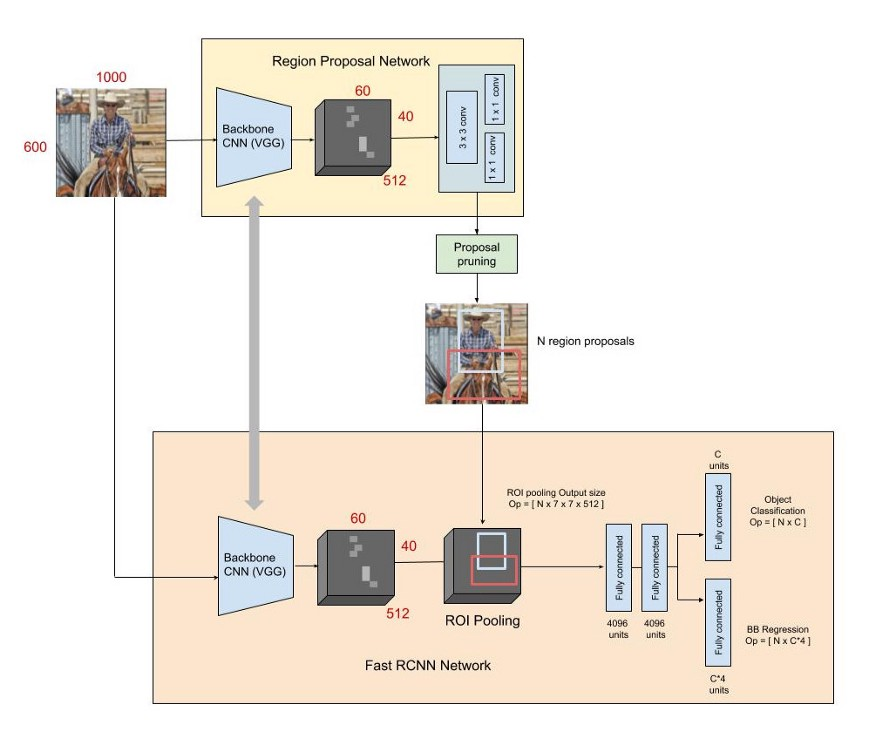
\includegraphics[scale=0.42]{graphics/fasterrcnn.jpeg}
  \caption{RPN cho các đề xuất khu vực và Fast R-CNN dưới dạng detector trong Faster R-CNN pipeline}
\end{figure}

Fast R-CNN cũng bao gồm một mạng CNN cơ bản, một lớp RoI pooling và các lớp fully connected được theo sau bởi hai nhánh đồng cấu trúc để thực hiện phân loại và hồi quy các bounding box.

Ảnh đầu vào trước tiên được truyền qua mạng CNN cơ bản để có trích xuất ra được feature map (Kích thước đặc trưng: 60, 40, 512). Bên cạch hiệu quả về thời gian thử nghiệm, một lý do quan trọng khác để sử dụng RPN như một công cụ tạo các vùng đề xuất là lợi ích của việc chia sẻ trọng số giữa mạng CNN của RPN và mạng CNN của Fast R-CNN.
Tiếp theo, các bounding box đề xuất từ RPN được sử dụng để tạo các đặc trưng từ feature map. Điều này được thực hiện bằng lớp RoI pooling. Lớp RoI pooling hoạt động bằng cách: Lấy vùng tương ứng với một đề xuất từ feature map; b) Chia vùng này thành một số cửa sổ con cố định; c) Thực hiện max-pooling trên các cửa sổ con này để tạo ra đầu ra có kích thước cố định.
Đầu ra từ lớp RoI pooling có kích thước (N, 7, 7, 512) trong đó N là số vùng đề xuất từ RPN. Sau khi chạy qua hai lớp fully connected, các đặc trưng được đưa vào các classification layer và regression layer.

Lưu ý rằng các nhánh classification và regression này khác với nhánh của RPN. Ở đây, classification layer có C đơn vị cho mỗi lớp trong mỗi lần phát hiện (bao gồm lớp background). Các đặc trưng được truyền qua lớp softmax để có được classification scores - xác suất của một vùng đề xuất thuộc về từng lớp. Các hệ số của regression layer được sử dụng để cải thiện việc dự đoán các bounding box. Ở đây, regression layer không phụ thuộc vào kích thước (không giống với RPN), nhưng phụ thuộc vào từng lớp. Điều đó có nghĩa là tất cả các lớp đều có regression layer riêng với 4 tham số mỗi lớp tương ứng với C*4 đơn vị đầu ra trong regression layer.

\paragraph{Lý do sử dụng Faster R-CNN cho bài toántoán\\}

Sau khi tìm hiểu về các mô hình như nhóm đã trình bày thì việc chọn Faster R-CNN làm mô hình để thực nghiệm cho bài toán nhận diện người đi bộ là một quyết định có cơ sở và hy vọng mang lại kết quả tốt trong việc giám sát và phân loại người đi bộ trong các môi trường thực tế. Từ biểu đồ sau đây, ta có thể thấy rằng, Faster R-CNN có hiệu suất tốt hơn rất nhiều so với các mô hình khác trong gia đình R-CNN. Đó cũng chính là lý do vì sao nhóm chọn mô hình này để thực nghiệm và đánh giá. 

\begin{figure}[h!]
  \centering
  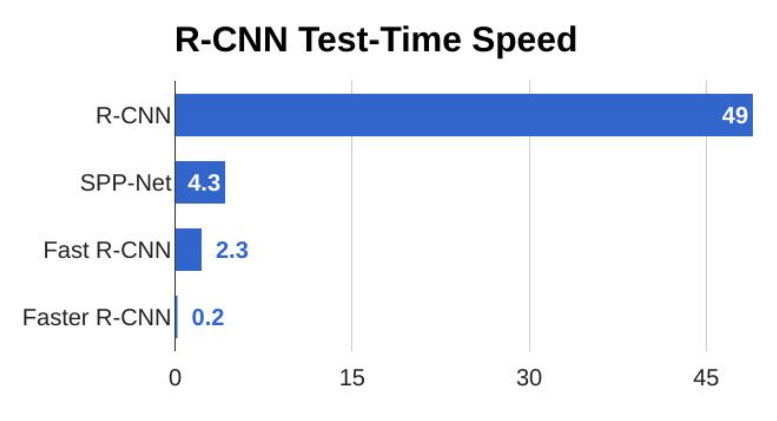
\includegraphics[scale=0.6]{graphics/whychoosefaster.png}
  \caption{Biểu đồ đánh giá về thời gian thực nghiệm của các mô hình họ R-CNN \cite{slide}}
\end{figure}

